\chapter*{Criação da API JSON}\label{sec:parte3}

A parte seguinte foi a criação da Rest API em JSON para permitir mostrar e trabalhar os dados na aplicação web.
\newline Para criar a API foi usado o RESTful Service que a Oracle disponibiliza no seu produto.

\begin{figure}[h!]
 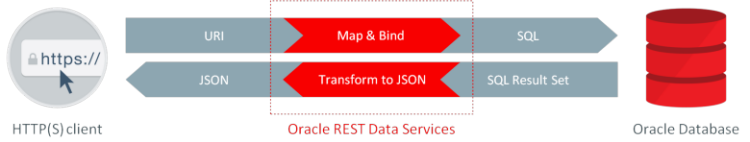
\includegraphics[width=\linewidth]{tex/figs/3606406.png}
    \caption{Esquema do RESTful Service} 
    \label{fig:esquemarest}
\end{figure}

Para ativar o serviço na Base de Dados por nós criado foi utilizado o SQL Developer e foi criado um script em SQL para ativar o serviço.
\newline Foram necessários os seguintes passos:
\begin{enumerate}
    \item Ativar o RESTful Service para a base de dados Mic;
    \item Ativar o RESTful Service para cada tabela;
\end{enumerate}
Estes passos foram utilizando a ligação do utilizador criado nos passos anteriores.
Posto isto, os scripts em SQL são os seguintes:


\textbf{Ativação para a base de dados}
\begin{lstlisting}
DECLARE
  PRAGMA AUTONOMOUS_TRANSACTION;
BEGIN

    ORDS.ENABLE_SCHEMA(p_enabled => TRUE,
                       p_schema => 'MIC',
                       p_url_mapping_type => 'BASE_PATH',
                       p_url_mapping_pattern => 'mic',
                       p_auto_rest_auth => FALSE);

    commit;

END;
\end{lstlisting}

\textbf{Ativação para as tabelas}
\begin{lstlisting}
DECLARE
  PRAGMA AUTONOMOUS_TRANSACTION;
BEGIN

    ORDS.ENABLE_OBJECT(p_enabled => TRUE,
                       p_schema => 'MIC',
                       p_object => <nome_da_tabela>,
                       p_object_type => 'TABLE',
                       p_object_alias => 'datafiles',
                       p_auto_rest_auth => FALSE);

    commit;

END;
\end{lstlisting}

Foi incluído um script SQL na pasta do projeto que depois de executado ativa o serviço tanto na base de dados como em todas as tabelas.

Depois disto o serviço REST ficou pronto a ser usado na aplicação web com os seguintes endpoints:
\begin{itemize}
    \item http://localhost:8080/ords/mic/tablespaces
    \item http://localhost:8080/ords/mic/tablespaceshistory
    \item http://localhost:8080/ords/mic/memory
    \item http://localhost:8080/ords/mic/datafiles
    \item http://localhost:8080/ords/mic/datafileshistory
    \item http://localhost:8080/ords/mic/io\_reads
    \item http://localhost:8080/ords/mic/tables
    \item http://localhost:8080/ords/mic/io\_writes
    \item http://localhost:8080/ords/mic/sessions
    \item http://localhost:8080/ords/mic/sessionshistory
    \item http://localhost:8080/ords/mic/users
    \item http://localhost:8080/ords/mic/usershistory
\end{itemize}

Com isto, demos por terminada a fase da preparação da API, tendo agora todo o conteúdo das tabelas da nossa base de dados disponível no formato JSON e pronto para criarmos a aplicação web.